\section{Discussion and Analysis}\label{sec:discussion}
\begin{figure*}[t]
    % (k, 1) CTDG
    \centering
    \begin{subfigure}[b]{0.23\textwidth}
        \centering
        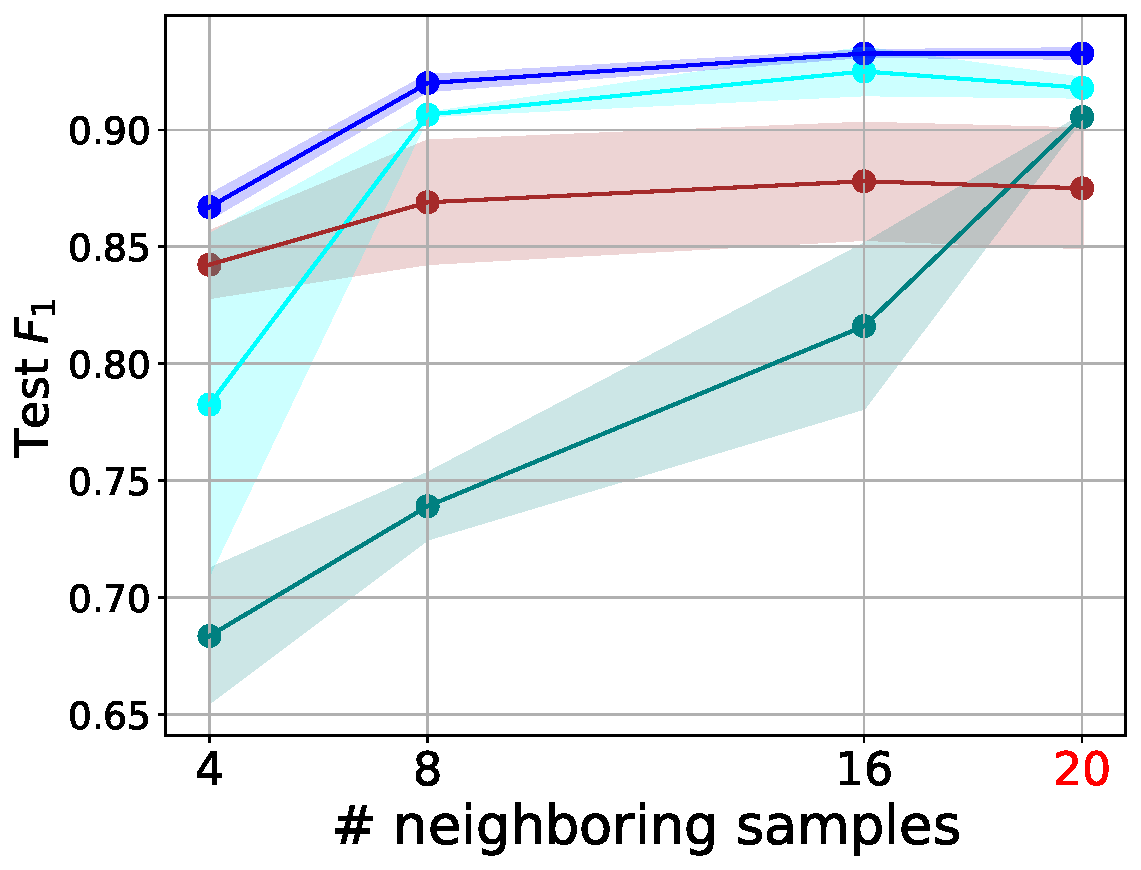
\includegraphics[width=\linewidth]{figs/periodicity/sbm_sto/V2/num_neighboring/multi_seed/(8,1)(0.9, 0.01).pdf}
        \caption{$\Psto{8, 1}$}
        \label{fig:sto_periodic_8_num_nei}
    \end{subfigure}
    \hfill
    \begin{subfigure}[b]{0.22\textwidth}
        \centering
        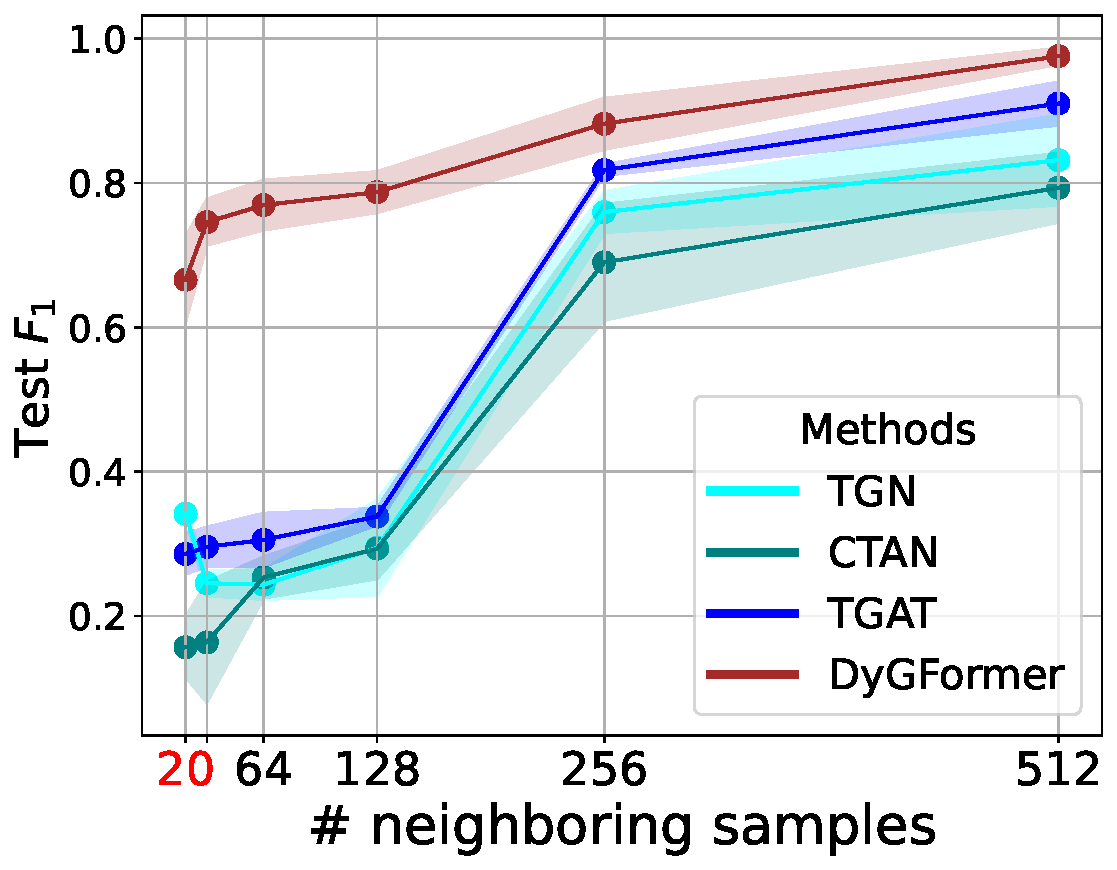
\includegraphics[width=\linewidth]{figs/periodicity/Fixed_ER/num_neighboring/multi_seed/(256,1).pdf}
        \caption{$\Pdet{256, 1}$}
        \label{fig:det_periodic_256_num_nei}
        \label{fig:sub_all_(k, 1)_(0.9, 0.01)_sbm_sto}
    \end{subfigure}
    \hfill
    \begin{subfigure}[b]{0.24\textwidth}
    \centering
    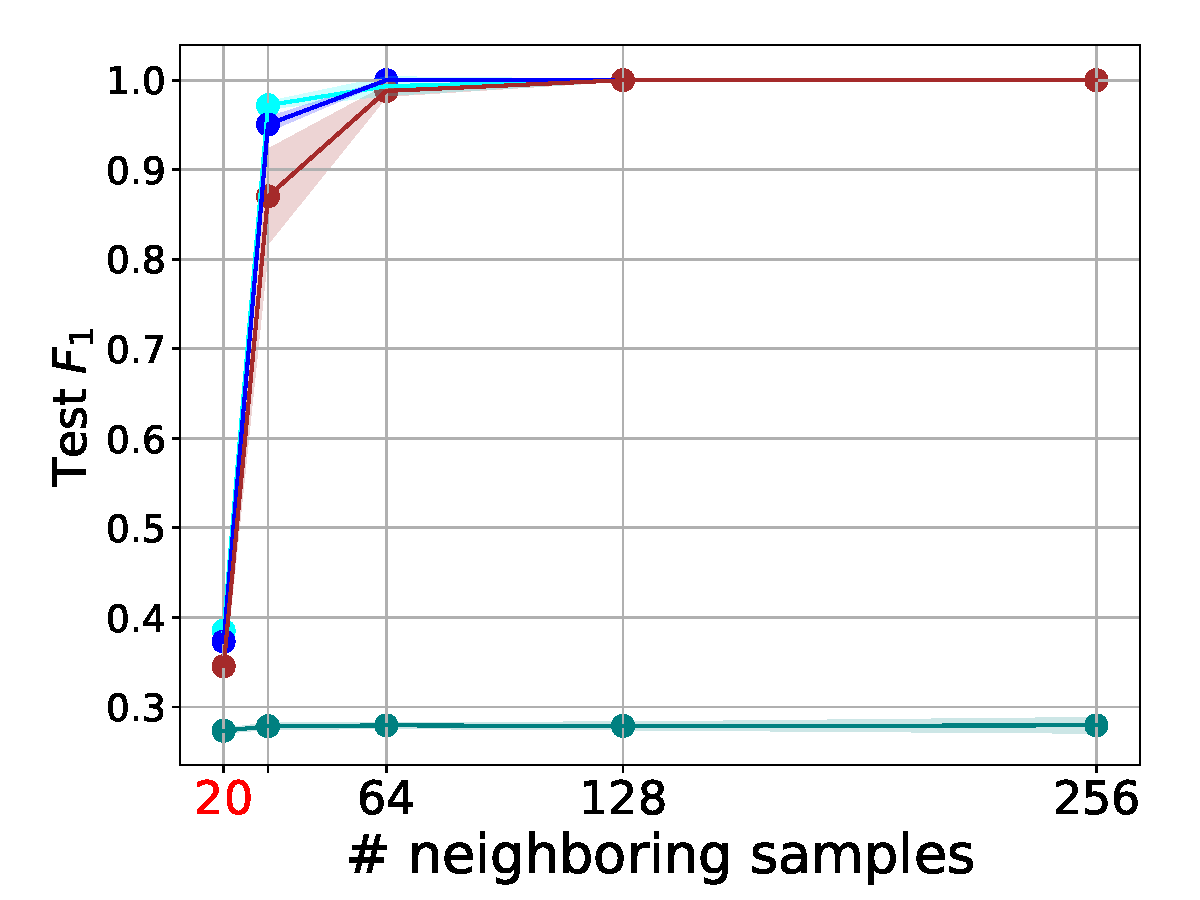
\includegraphics[width=\linewidth]{figs/memory_node/num_neighbors/(64,4000).pdf}
    \caption{$\causeeffect{64}$}
    \label{fig:cause_effect_64_num_nei}
    \end{subfigure}
    \begin{subfigure}[b]{0.24\textwidth}
    \centering
    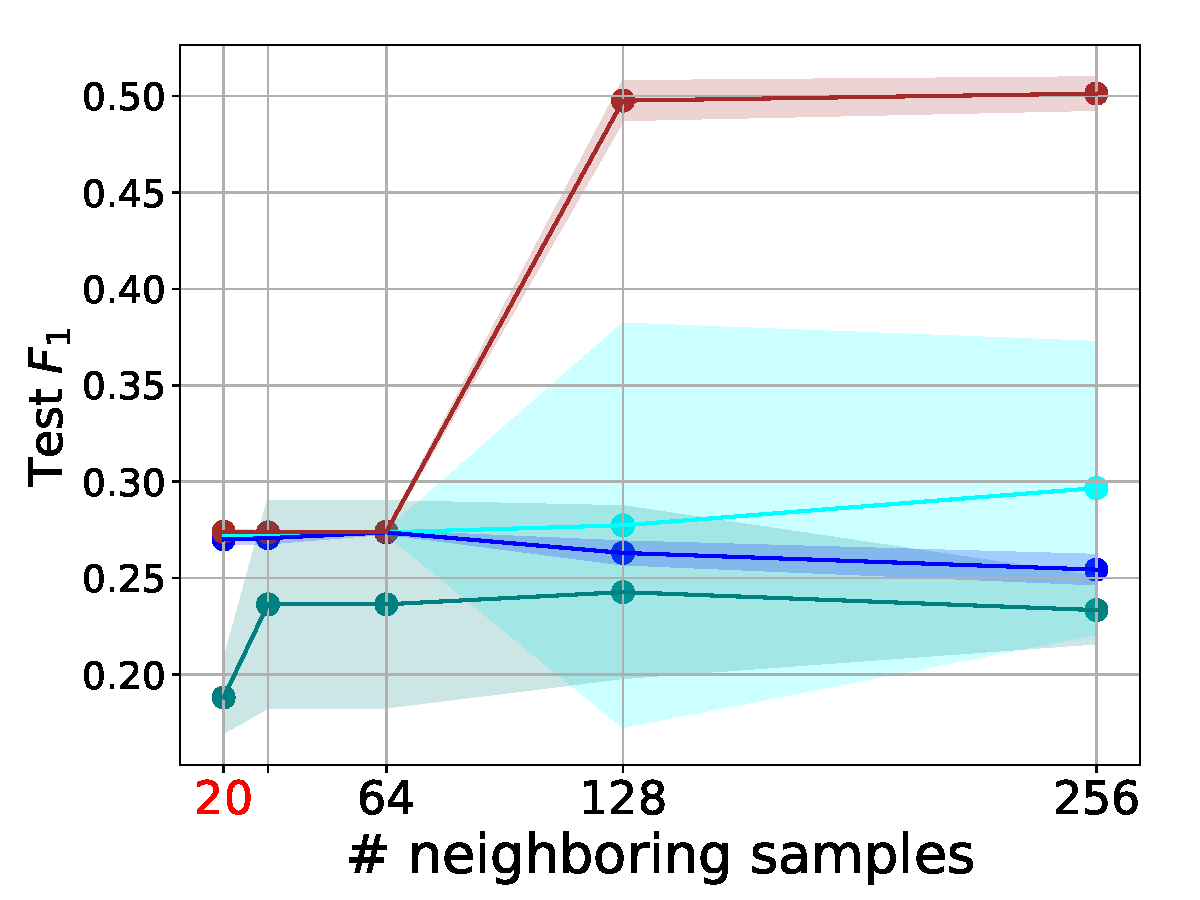
\includegraphics[width=\linewidth]{figs/memory_node/num_neighbors/(256,4000).pdf}
    \caption{$\causeeffect{256}$}
    \label{fig:cause_effect_256_num_nei}
    \end{subfigure}
    
    \caption{Effect of the number of neighbors on periodic (left), and cause-and-effect (right) tasks .}
    \label{fig:multi_seed_neighbors}
\end{figure*}

\begin{table*}[t]
\centering
\caption{Average method rank~($\downarrow$) for \benchmarkname tasks~(c.p. stands for change points). Top results are shown in \first{first}, \second{second}, \third{third}.} \label{tab:overall}
\resizebox{0.7\linewidth}{!}{%
\begin{tabular}{l l |ccccc|c|cccc}
\toprule
 %\multirow{2}{*}{ %\diagbox{Name}{Data} 
 % \begin{tabular}{l}
 %      \hspace*{0.75cm}Dataset \\
 %      Models
 % \end{tabular}

 %  \begin{tabular}{l}
 %      Models
 % \end{tabular}
 %} 
&& \multicolumn{5}{c|}{Periodicity} & Cause \& & \multicolumn{4}{c}{Long-Range Dependencies} \\
& Method & \multicolumn{2}{c}{$\Pdet{2,n}$} &\multirow{2}{*}{$\Pdet{k,1}$} & \multicolumn{2}{c|}{$\Psto{2,n}$} & Effect &  \multicolumn{4}{|c}{$\longrange{\lag,d}$} \\    
& & all $t$  & c.p. &  & $p=0.5$ & $p=0.9$ & $\causeeffect{\ell}$ & $\lag\!=\!1$ & $\lag\!=\!4$ & $\lag\!=\!16$ & $\lag\!=\!32$ \\ 
%
%
%  & \multirow{2}{*}{Method}& \multicolumn{5}{c|}{Periodicity} & \multicolumn{1}{c|}{
% \begin{tabular}{@{}c@{}}Cause \& \\ Effect\end{tabular}
% } & \multicolumn{4}{c}{Spatio-temporal long-range} \\   
%     & & $(2, n)$ - A & $(2, n)$ - C & $(k, 1)$ & $(0.5)$ & $(0.9)$ & $\causeeffect{\ell}$ & $(1, d)$ & $(4, d)$ & $(16, d)$ & $(32, d)$ \\ 
  \midrule

  \multirow{4}{*}{\rotatebox[origin=c]{90}{CTDG}} & 
  CTAN & 5.625 & \third{3.75} & 7.625 & \second{3.167} & 5.167 & 6.4 & 10.0 & 8.6 & 8.4 & 6.8 \\
  & DyGFormer & \second{3.25} & \second{3.5} & \third{2.625} & 7.167 & 7.5 & \third{3.2} & \second{2.2} & \second{1.8} & \third{3.0} & \second{3.4} \\
  & TGAT & 4.75 & 5.0 & 4.375 & \third{3.667} & \second{3.167} & \second{2.6} & 3.8 & \first{1.6} & \first{1.0} & \first{1.8} \\
  & TGN & 5.75 & 7.125 & 4.625 & \third{3.667} & 4.33 & \first{2.4} & 4.8 & \third{2.8} & \second{2.0} & \first{1.8} \\
  \midrule
  \multirow{5}{*}{\rotatebox[origin=c]{90}{DTDG}} 
  & GC-LSTM & \first{2.875} & \first{3.125} & \first{1.25} & \first{1.0} & \first{1.167} & 4.8 & \third{3.0} & 4.6 & 5.6 & 6.2 \\
  & EGCN & 10.875 & 10.0 & 9.75 & 6.5 & 8.167 & 5.0 & 8.2 & 7.8 & 7.0 & 8.0 \\
  & T-GCN & \second{3.25} & \third{3.75} & \second{2.5} & 6.5 & \third{3.333} & 9.6 & \first{1.8} & 4.2 & 4.8 & \third{6.0}\\
  & GCN & 8.875 & 8.0 & 7.0 & 9.833 & 9.833 & 7.8 & 6.8 & 8.8 & 9.2 & 9.0 \\
  & GAT & 7.625 & 6.5 & 6.0 & 7.5 & 5.333 & 8.0 & 5.6 & 8.6 & 8.2 & 6.4 \\
  \midrule
  & EdgeBank & 8.5 & 4.25 & 9.25 & 6.0 & 7.0 & 5.2 & 8.8 & 6.0 & 5.4 & 9.8 \\
  & Persistence & \third{4.625} & 11.0 & 11.0 & 11.0 & 11.0 & 11.0 & 11.0 & 11.0 & 11.0 & 11.0 \\
  % \texttt{tgbl-wiki} &  9,227 - 56756 & 157,474 & 18,257 &  152,757 & 0.108 & 1 month\\ 
  % Reddit & 10,984 & 672,447 & 78,516 & 669,065 & 0.069 & 1 month  \\  
  % LastFM & 1,980 & 1,293,103 & 154,993 & 1,283,614 &  0.35 & 1 month \\
  % UCI & 1,899 & 26,628 & 20,296 & 58,911 & 0.535 & 196 days \\
  % Enron & 184 & 10,472 & 3,125 & 22,632 & 0.253 & 3 years \\
  \bottomrule
\end{tabular}
}
\end{table*}






% % single vs. multiple layer comparison ranking on long-range dependency
% \begin{table*}[t]
% \centering
% \caption{Average method rank~($\downarrow$) ,one- vs. tw o-layer setting, for \benchmarkname. Top results are shown in \first{first}, \second{second}, \third{third}.} \label{tab:overall}
% \resizebox{0.7\linewidth}{!}{%
% \begin{tabular}{l l |ccc|ccc}
% \toprule
%  %\multirow{2}{*}{ %\diagbox{Name}{Data} 
%  % \begin{tabular}{l}
%  %      \hspace*{0.75cm}Dataset \\
%  %      Models
%  % \end{tabular}

%  %  \begin{tabular}{l}
%  %      Models
%  % \end{tabular}
%  %} 
% && \multicolumn{6}{c}{Long-Range Dependencies} \\
% & Method &  \multicolumn{3}{|c}{$\longrange{\lag,d}$}  &  \multicolumn{3}{|c}{$\longrange{\lag,d}$} \\  
% & & \multicolumn{3}{c}{one-layer} & \multicolumn{3}{|c}{two-layer} \\
% & & $\lag\!=\!1$ & $\lag\!=\!4$ & $\lag\!=\!16$ & $\lag\!=\!1$ & $\lag\!=\!4$ & $\lag\!=\!16$ \\ 
% %
% %
% %  & \multirow{2}{*}{Method}& \multicolumn{5}{c|}{Periodicity} & \multicolumn{1}{c|}{
% % \begin{tabular}{@{}c@{}}Cause \& \\ Effect\end{tabular}
% % } & \multicolumn{4}{c}{Spatio-temporal long-range} \\   
% %     & & $(2, n)$ - A & $(2, n)$ - C & $(k, 1)$ & $(0.5)$ & $(0.9)$ & $\causeeffect{\ell}$ & $(1, d)$ & $(4, d)$ & $(16, d)$ & $(32, d)$ \\ 
%   \midrule

%   \multirow{2}{*}{\rotatebox[origin=c]{90}{CTDG}} & \\
%   & DyGFormer &\second{2.2} & \second{1.8} & \third{3.0} & 2.8 & \second{1.8} & \second{2.0} \\
%    & TGAT & 3.8 & \first{1.6} & \first{1.0} & \first{2.2} & \first{1.2} & \first{1.0} \\
%   & TGN & 4.8 & \third{2.8} & \second{2.0} & 5.0 & 5.0 & 5.0 \\
%   \midrule
%   \multirow{2}{*}{\rotatebox[origin=c]{90}{DTDG}} 
%   & GC-LSTM & \third{3.0} & 4.6 & 5.6 & \second{2.4} & \third{3.2} & 4.2 \\
%   & T-GCN & \first{1.8} & 4.2 & 4.8 & \third{2.6} & 3.8 & \third{4.0} \\
%   \midrule
%   % Reddit & 10,984 & 672,447 & 78,516 & 669,065 & 0.069 & 1 month  \\  
%   % LastFM & 1,980 & 1,293,103 & 154,993 & 1,283,614 &  0.35 & 1 month \\
%   % UCI & 1,899 & 26,628 & 20,296 & 58,911 & 0.535 & 196 days \\
%   % Enron & 184 & 10,472 & 3,125 & 22,632 & 0.253 & 3 years \\
%   \bottomrule
% \end{tabular}
% }
% \end{table*}


In this section, we synthesize key findings and insights across all three task categories in T-GRAB.

\textbf{Bird's eye view of the results.} Table~\ref{tab:overall} presents a comprehensive ranking of methods across our benchmark tasks. \ad{ For each task, each method is ranked by averaging the performance scores across all tested parameter settings, each of which is obtained by averaging over multiple seeds.}
Our analysis reveals a striking dichotomy in model effectiveness across different temporal reasoning challenges. For periodicity tasks, GC-LSTM consistently outperforms all competitors across all five settings, challenging the prevailing assumption that CTDG methods outperform DTDG ones~\cite{huangutg}. This suggests that for tasks requiring precise counting and pattern memorization, the simpler recurrent architecture of DTDG models may offer computational advantages over their more complex continuous-time counterparts. Conversely, for cause-and-effect and long-range dependencies tasks, CTDG methods, particularly TGN and TGAT emerge as the dominant methods. Notably, CTAN, despite being explicitly designed for long-range temporal propagation, performs surprisingly poorly on the long-range dependencies tasks. This unexpected result highlights potential limitations in its ability to \textit{jointly reason} over spatial and temporal dimensions.

\looseness-1 These findings collectively demonstrate that no single architectural paradigm excels across all \benchmarkname tasks. The observed performance variations suggest that different architectural inductive biases are better suited to specific temporal reasoning challenges. This insight points to a promising research direction: developing hybrid architectures that can effectively combine the strengths of different approaches to achieve superior performance across diverse temporal reasoning scenarios.

\looseness-1 \textbf{Effect of Number of Neighbors.} Temporal neighbor sampling is a fundamental mechanism in CTDG methods~\cite{dygformer,tgn,tgat,luo2022neighborhood}, that allows  models to access historical interactions and model temporal dependencies, especially crucial in scenarios with sparse edge distributions. Despite its importance, the number of sampled neighbors remains an under-examined hyperparameter, commonly fixed at default values (e.g., 20 neighbors in established literature~\cite{dygformer}). We maintained this conventional setting in our previous experiments but now systematically investigate how this parameter influences performance across \benchmarkname tasks.

\looseness-1 Figures~\ref{fig:sto_periodic_8_num_nei} and~\ref{fig:det_periodic_256_num_nei} illustrate performance on periodic tasks as a function of neighbor count. Our analysis reveals that CTAN, TGN, and TGAT exhibit pronounced performance improvements with increased neighbor sampling across both stochastic and deterministic settings, demonstrating their substantial sensitivity to this parameter. For DyGFormer, this parameter directly determines the temporal context length for sequence construction, and it maintains relatively consistent performance, suggesting a more robust architecture with respect to neighbor sampling. 
% Additional analyses are available in Appendix~\ref{apendix:neighbours}. 


Extending our 
investigation to cause-and-effect tasks (Figures~\ref{fig:cause_effect_64_num_nei} and~\ref{fig:cause_effect_256_num_nei}), we observe that for $\causeeffect{64}$, TGAT, TGN, and DyGFormer continue to benefit from sampling beyond 32 neighbors, while CTAN plateaus, indicating a fundamental limitation in its capacity and design. For the more challenging $\causeeffect{256}$ task, DyGFormer demonstrates continued improvement with larger neighbor counts (particularly beyond 128), while other methods reach performance saturation. These findings suggest potential for further performance gains through even larger sampling windows (e.g., 512 neighbors), albeit with corresponding computational overhead.

\looseness-1 \textbf{Limitations.}
\changed{
While \benchmarkname serves as a valuable diagnostic tool for probing specific temporal reasoning capabilities of TGNNs, it is not intended to replace real-world benchmarks. Much like the CLEVR dataset in computer vision~\cite{clevr}, our benchmark offers a controlled environment that isolates fundamental temporal patterns, enabling us to rigorously assess the extent to which TGL models can learn and generalize such patterns. Good performances on \benchmarkname is not guaranteed to directly translate to real world dataset, and to obtain a comprehensive understanding of model performance in practical applications, it is essential to complement T-GRAB with evaluations on real-world datasets exhibiting complex dynamics, noise, and heterogeneity.}

\changed{Another limitation is our focus on discrete time graphs. This choice is motivated by the fact that discrete time graphs offers a cleaner and more interpretable setting, making it the simplest and most fair choice for benchmarking both DTDG and CTDG methods on core reasoning skills. Extending \benchmarkname to continuous time graphs is non-trivial and would require decisions about sampling timestamps from continuous intervals, handling event sparsity, and maintaining fair comparisons across fundamentally different modeling paradigms~\cite{huangutg}. Moreover, evaluations relying on fine-grained temporal dependencies are inherently limited by the resolution of the discrete time setup, making them less suited for benchmarking models that operate in truly continuous-time settings. As such, extending \benchmarkname tasks to continuous time graphs in future work will be crucial for fully capturing the breadth of temporal graph learning challenges.
}

% \textbf{Effect of number of neighbors}
% Sampling temporal neighbors is a key procedure in many CTDG methods~\cite{dygformer,tgn,tgat,luo2022neighborhood}, enabling models to retrieve past interactions and capture temporal dependencies. This is required in CTDG methods as the number of edges at any given fine-grained timestamp is often very low thus, retrieving past interaction information is crucial for learning. How many temporal neighbors to sample thus becomes an important hyperparameter to consider. More sampled neighbours mean interactions from longer timestamps ago are included, often with trade-offs in computational cost. However, the number of temporal neighbors is often left at the default value and is less explored in prior work. In all our experiments thus far, we followed the common practice of using 20 historical neighbors~\cite{dygformer}. Here, we explore the effect of the number of temporal neighbors on \benchmarkname tasks. 

% \textbf{Periodic Task Observations.} Figure~\ref{fig:det_periodic_256_num_nei} and Figure~\ref{fig:sto_periodic_8_num_nei} illustrate our investigation into how the number of historical neighbors influences model performance on the periodic tasks we designed. In the case of DyGFormer, this parameter directly corresponds to the context length, since the model samples temporal neighboring nodes to form a temporal sequence for input. Interestingly, our results reveal that increasing the number of historical neighbors substantially improves the performance of CTAN, TGN, and TGAT in both stochastic and deterministic settings, highlighting how sensitive these models are to the richness of historical context. In contrast, DyGFormer exhibited a notably more stable performance, indicating a lower dependency on the number of neighboring samples during training. This distinction underscores the importance of understanding and tuning this often-overlooked hyperparameter in temporal graph learning models. Additional experiments supporting our findings on the influence of neighboring samples are provided in~\ref{apendix:neighbours}.

% \textbf{Delayed Cause-and-Effect Task Observations.}
% As shown in figure~\ref{fig:cause_effect_64_num_nei} and~\ref{fig:cause_effect_256_num_nei}, we extended our investigation to the cause-and-effect task. On $\causeeffect{64}$, increasing the number of neighboring samples beyond 32 continued to show a notable positive impact on the performance of TGAT, TGN, and DyGFormer. In contrast, CTAN’s performance remained unchanged, highlighting its limitations in modeling temporal cause-and-effect relationships. Moving to $\causeeffect{256}$, DyGFormer’s performance continued to improve with more neighbors, particularly after 128, while the other methods appeared to plateau. For these methods, we suggest exploring even higher neighbor counts, such as 512 or more, which could potentially enhance performance, albeit with additional training cost.

% Temporal information from neighboring samples plays a crucial role in temporal graph learning \ad{some citations}, enabling models to capture dynamic patterns and temporal dependencies as the graph evolves. One important factor is the number of historical neighboring samples considered, which can enrich the model’s temporal context but comes with trade-offs in terms of increased computational cost and training time. Despite its importance, to the best of our knowledge, the impact of the number of historical neighboring samples has not been systematically examined in temporal graph learning. In all our experiments thus far, we followed the common practice of using 20 historical neighbors \ad{bring some citations here, like DyGFormer, etc} and reported the results accordingly. In this section, we extend this investigation by exploring how varying this number both lower and higher, influences the performance of CTDG methods. 

% \textbf{Effect of Neighbours in Periodic Tasks.}
% Figure~\ref{fig:det_periodic_256_num_nei} and Figure~\ref{fig:sto_periodic_8_num_nei} illustrate our investigation into how the number of historical neighbors influences model performance on the periodic tasks we designed. In the case of DyGFormer, this parameter directly corresponds to the context length, since the model samples temporal neighboring nodes to form a temporal sequence for input. Interestingly, our results reveal that increasing the number of historical neighbors substantially improves the performance of CTAN, TGN, and TGAT in both stochastic and deterministic settings, highlighting how sensitive these models are to the richness of historical context. In contrast, DyGFormer exhibited a notably more stable performance, indicating a lower dependency on the number of neighboring samples during training. This distinction underscores the importance of understanding and tuning this often-overlooked hyperparameter in temporal graph learning models.

% \textbf{Effect of Neighbours in Delayed Cause-and-Effect Tasks.} As shown in figure~\ref{fig:cause_effect_64_num_nei} and~\ref{fig:cause_effect_256_num_nei}, we extended our investigation to the cause-and-effect task. On $\causeeffect{64}$, increasing the number of neighboring samples beyond 32 continued to show a notable positive impact on the performance of TGAT, TGN, and DyGFormer. In contrast, CTAN’s performance remained unchanged, highlighting its limitations in modeling temporal cause-and-effect relationships. Moving to $\causeeffect{256}$, DyGFormer’s performance continued to improve with more neighbors, particularly after 128, while the other methods appeared to plateau. For these methods, we suggest exploring even higher neighbor counts, such as 512 or more, which could potentially enhance performance, albeit with additional training cost. 


% \begin{figure}[H]
% \begin{figure}[t]
%     % (k, 1) CTDG
%     \centering
%     \begin{subfigure}[b]{0.255\textwidth}
%     \centering
%     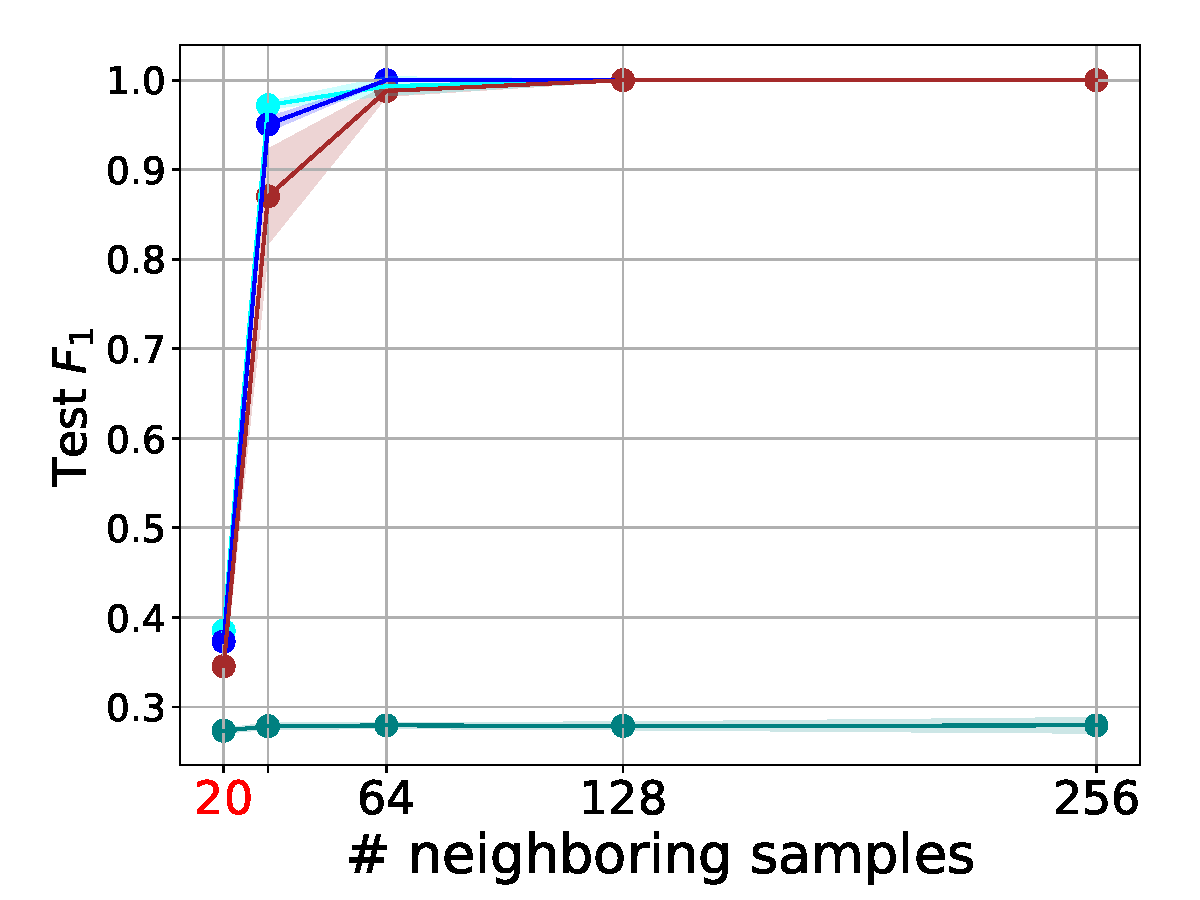
\includegraphics[width=\linewidth]{figs/memory_node/num_neighbors/(64,4000).pdf}
%     \caption{$\causeeffect{64}$}
%     \label{fig:cause_effect_64_num_nei}
%     \end{subfigure}
%     \begin{subfigure}[b]{0.255\textwidth}
%     \centering
%     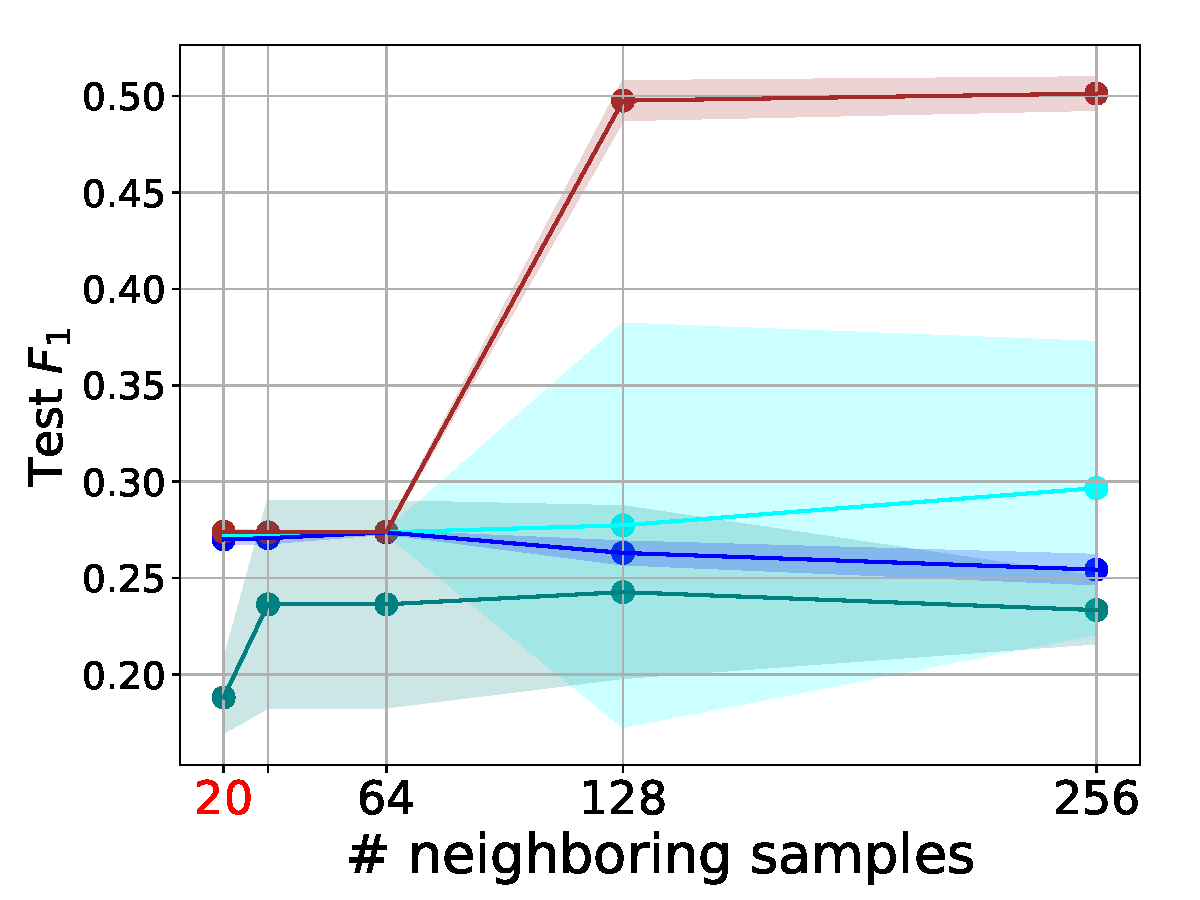
\includegraphics[width=\linewidth]{figs/memory_node/num_neighbors/(256,4000).pdf}
%     \caption{$\causeeffect{256}$}
%     \label{fig:cause_effect_256_num_nei}
%     \end{subfigure}
%     \begin{subfigure}[b]{0.24\textwidth}
%         \centering
%         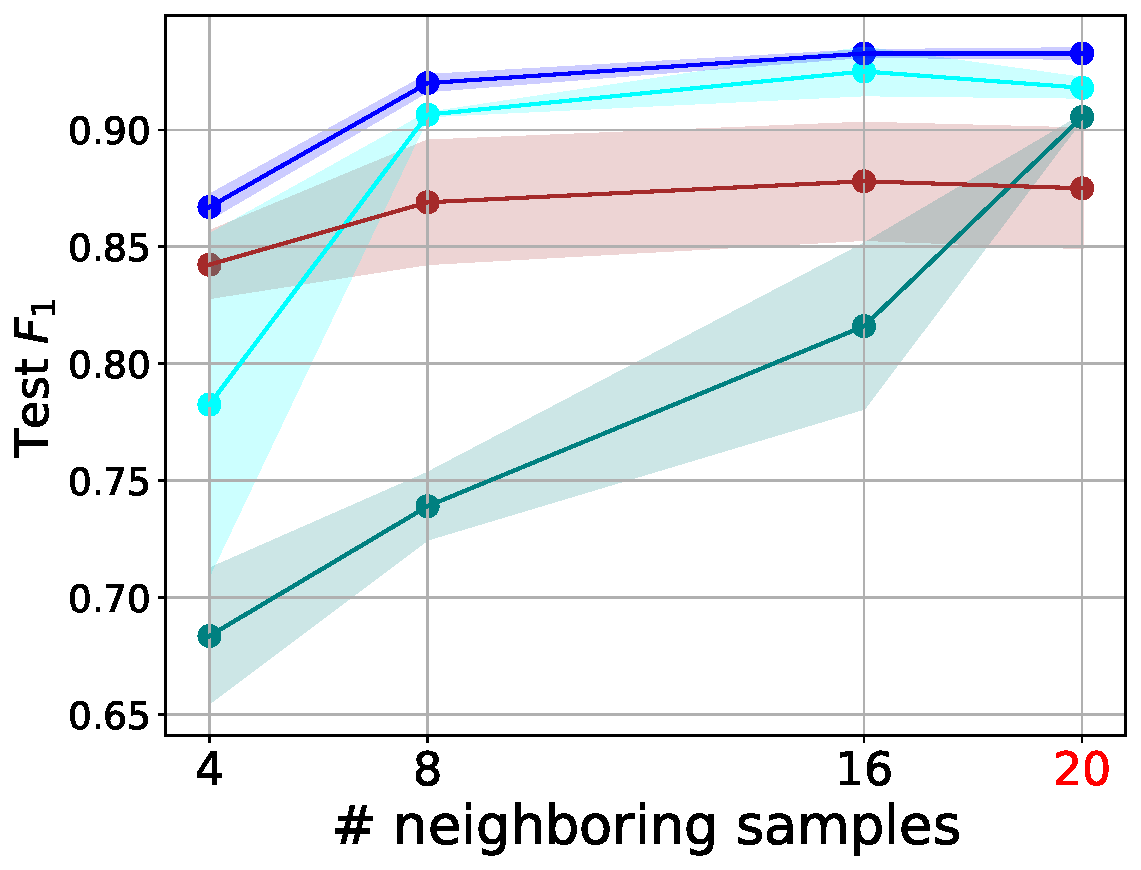
\includegraphics[width=\linewidth]{figs/periodicity/sbm_sto/V2/num_neighboring/multi_seed/(8,1)(0.9, 0.01).pdf}
%         \caption{$\Psto{8, 1}$}
%         \label{fig:sto_periodic_8_num_nei}
%     \end{subfigure}
%     \hfill
%     \begin{subfigure}[b]{0.23\textwidth}
%         \centering
%         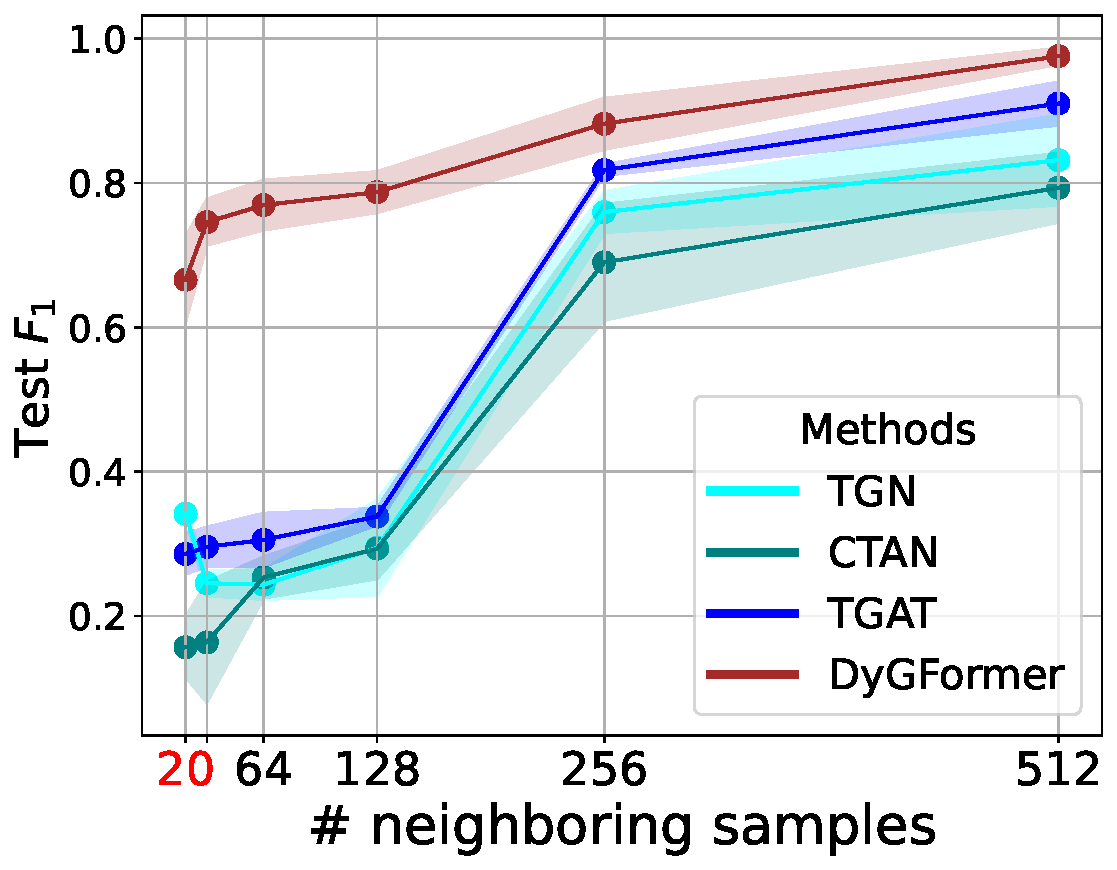
\includegraphics[width=\linewidth]{figs/periodicity/Fixed_ER/num_neighboring/multi_seed/(256,1).pdf}
%         \caption{$\Pdet{256, 1}$}
%         \label{fig:det_periodic_256_num_nei}
%         \label{fig:sub_all_(k, 1)_(0.9, 0.01)_sbm_sto}
%     \end{subfigure}
    
%     \caption{Impact of the number of neighboring samples on cause-and-effect and periodic tasks.}
%     \label{fig:multi_seed_neighbors}
% \end{figure}



% For further investigation, This motivates us to train TGN with three different number of neighbors, as depicted at Figure~\ref{fig:(K,1)_TGN}: the default 20 ("TGN"), a size equal to the period length ("TGN-K"), and double the period length ("TGN-2K"). Empirically, TGN performs significantly better when using twice the period length, surpassing both the default 20 and the same-size period settings. \\





